\subsection{Động lượng}
\begin{frame}
    \frametitle{Hệ chất điểm}
    Hệ chất điểm là tập hợp của \(N\) chất điểm \(M_i\) có khối lượng \(m_i\) và vận tốc \(\mathbf{v}_i\), \(i=1,2,\ldots,N\).

    Ta định nghĩa khối tâm \(G\) của hệ chất điểm là điểm sao cho
    \begin{equation}
    \Sigma_i m_i \mathbf{GM_i} = 0.
    \end{equation}
    Khi đó,
    \begin{equation}
    \mathbf{OG} = \frac{\Sigma_i m_i \mathbf{OM_i}}{m}.
    \end{equation}
    và
    \begin{equation}
        \mathbf p=\Sigma_i m_i \mathbf{v}_i = m\mathbf{v_G}.
    \end{equation}
    Trong đó \(m=\Sigma_i m_i\) và \(\mathbf p\) là khối lượng và động lượng toàn phần của hệ.
\end{frame}

\begin{frame}
    \frametitle{Định luật II Newton cho hệ chất điểm}
    Định luật II Newton cho hệ chất điểm:
    \begin{equation}
        \frac{d\mathbf p}{dt} = \Sigma_i \mathbf{F}_i + \Sigma_i \Sigma_{j\neq i} \mathbf{f}_{ij}.
    \end{equation}
    Trong đó \(\mathbf{F}_i\) là ngoại lực tác dụng lên \(M_i\), và \(\mathbf{f}_{ij}\) là lực do \(M_j\) tác dụng lên \(M_i\).

    Số hạng thứ hai trong vế phải bằng 0 do định luật III Newton:
    \begin{equation}
        \frac{d\mathbf p}{dt}=\Sigma_i \mathbf{F}_i=m\mathbf{a_G}.
    \end{equation}
    Nếu tổng hợp lực ngoài tác dụng lên hệ bằng không, thì động lượng toàn phần của hệ được bảo toàn:
        \begin{equation}
            \mathbf p = \textbf{const}.
        \end{equation}
\end{frame}
\subsection{Động lượng góc-mô men động lượng}

\begin{frame}
    \frametitle{Mô men động lượng}
    Mô men động lượng \(\mathbf{L}\) của một hạt quanh một điểm \(O\) được định nghĩa bởi:
    \begin{equation}
        \mathbf{L}=\mathbf{r}\times\mathbf{p}.
    \end{equation}
    Trong đó \(\mathbf{r}\) là toạ độ của hạt so với điểm \(O\).
    Mô men động lượng của một hệ chất điểm là tổng mô men động lượng của các chất điểm trong đó:
    \begin{equation}
        \mathbf{L}=\Sigma_i \mathbf{r_i}\times\mathbf{p_i}.
    \end{equation}
    Nếu nội lực trong hệ do các chất điểm tác dụng lên nhau là lực xuyên tâm, và \(\mathbf{r_i}\times\mathbf{F_i}=\mathbf 0\), mô men động lượng của hệ được bảo toàn:
    \begin{equation}
        \mathbf{L}=\textbf{const}.
    \end{equation}
\end{frame}

\begin{frame}
\frametitle{Bài toán tên lửa}
Xét một tên lửa có tổng khối lượng \(m\) đang bay trong vũ trụ với vận tốc \(v\). Nhiên liệu được phóng ra sau một cách từ từ với vận tốc \(u\) so với tên lửa. Tính độ tăng vận tốc của tên lửa sau khi nó xả được một khối lượng nhiên liệu \(\Delta m\).
\vspace{1cm}
\begin{figure}
    \centering
    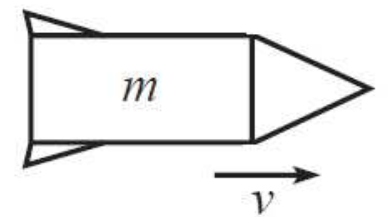
\includegraphics[width=0.3\textwidth]{Content/Figure/rocket.png}
\end{figure}
\end{frame}

\begin{frame}
\frametitle{Bài toán tên lửa}
\begin{columns}
\begin{column}{0.5\textwidth}
\begin{figure}
    \centering
    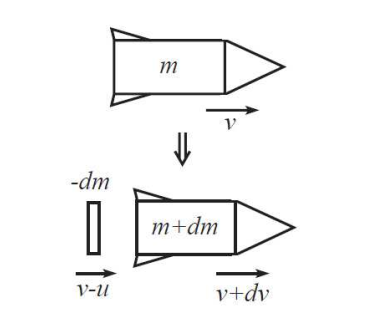
\includegraphics[width=0.6\textwidth]{Content/Figure/rocketsolving.png}
\end{figure}
Áp dụng định luật bảo toàn động lượng:
\begin{equation*}
    mv = (m+ dm)(v+dv) + (-dm)(v-u).
\end{equation*}
\end{column}
\begin{column}{0.5\textwidth}
    Ta suy ra được tích phân:
    \begin{equation}
        \int_{v}^{v+\Delta v} dv =- u \int_{m}^{m-\Delta m} \frac{dm}{m}.
    \end{equation}
    Từ đó ta thu được \(\Delta v\):
    \begin{equation}
        \Delta v = u \ln{\frac{m}{m-\Delta m}}.
    \end{equation}
\end{column}
\end{columns}
\end{frame}